\section{Описание алгоритма и стуктур данных}

Ориентированный граф представлен классом \verb|Graph|.
Вершины графа являются объектами класса \verb|Vertex|.

Вершина графа содержит имя и список ссылок на соседние вершины.
Список соседей хранится в виде ассоциативного массива 
пар (вершина -- вес ребра). 
То есть вот такой список соседей для вершины \verb|A|:

\begin{lstlisting}
{
    'B': 12,
    'C': 42,
    'D': -3,
}
\end{lstlisting}

на графе будет выглядеть так:

\begin{figure}[H]
    \centering
    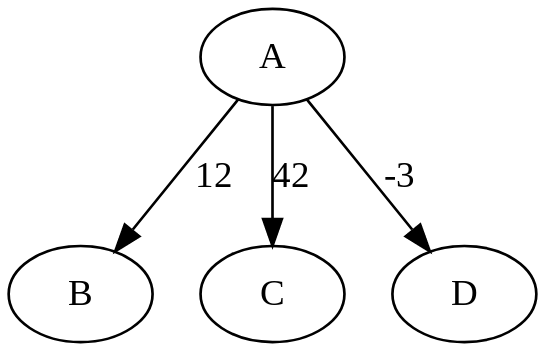
\includegraphics[width=0.7\linewidth]{photo/neighbors_example}
    \caption{Пример отображения соседей вершины графа}
    \label{fig:neighbors_example}
\end{figure}

Класс \verb|Graph| хранит вершины так же в виде ассоциативного массива 
пар (имя вершины -- объект вершины).

В упрощённом виде такая структуры хранения вершин и их связей
является списком смежности.

Граф можно загружать из файла.
Файл должен быть в формате:

\begin{verbatim}
Город_отправления_1;Город_прибытия_1;цена_перелета_1;цена_обратного_перелета_1
Город_отправления_2;Город_прибытия_2;цена_перелета_2;цена_обратного_перелета_1
...
Город_отправления_N;Город_прибытия_N;цена_перелета_N;цена_обратного_перелета_N
\end{verbatim}

Граф умеет находить минимальный путь от одной вершины до другой 
с помощью алгоритма Дейкстры. 
Алгоритм запускается для стартовой вершины и 
возвращает список минимальных путей и их значений.
Из полученных данных составляется последовательность
вершин, являющеюся минимальным маршрутом.
Полученная последовательность и её значение возвращаются.
